\chapter{Contexte Général et Cadre Méthodologique}
\section*{Introduction}
\addcontentsline{toc}{section}{Introduction}

Ce premier chapitre pose le cadre du projet Smart Farm AI : présentation
de l'entreprise d'accueil, analyse du contexte agricole tunisien, étude
de l'existant, définition des objectifs et description de la méthodologie
adoptée.

% ── 1.1 Organisme d'accueil ─────────────────────────────────
\section{Organisme d'accueil : Intech Solutions}

\subsection{Présentation générale}
\textbf{Intech Solutions} est une entreprise tunisienne de services numériques
spécialisée dans le développement de solutions intelligentes pour les secteurs
agro-industriels et agroalimentaires. Fondée à Sfax, elle s'est positionnée
sur le créneau porteur de l'agri-tech nationale en proposant des solutions
IoT, des plateformes SaaS et des services d'intégration IA adaptés aux
contraintes des exploitations tunisiennes.

\subsection{Domaines d'expertise}
\begin{itemize}
  \item Développement de plateformes SaaS multi-tenant pour la gestion d'exploitations ;
  \item Intégration IoT (microcontrôleurs ESP32, capteurs terrain, MQTT) ;
  \item IA appliquée : vision par ordinateur, NLP en langue arabe/Darija, modèles prédictifs ;
  \item Déploiement cloud souverain (Docker, Caddy, serveurs locaux) ;
  \item Applications mobiles PWA offline-first pour les zones à connectivité limitée.
\end{itemize}

\subsection{Vision stratégique}
La vision d'Intech Solutions s'articule autour du concept de
\textbf{souveraineté numérique agricole} : offrir aux agriculteurs tunisiens
des outils performants, économiques (open-source), en leur langue maternelle,
sans dépendance vis-à-vis des API propriétaires étrangères. Cette vision
a directement guidé les choix architecturaux du projet (Ollama local,
modèles embarqués, RBAC strict).

% ── 1.2 Contexte du projet ──────────────────────────────────
\section{Contexte et problématique}

\subsection{Étude de l'existant}

\begin{table}[H]
\centering
\caption{Comparaison des solutions Smart Farming existantes}
\label{tab:comparaison_existant}
\begin{tabularx}{\linewidth}{Xccccc}
\toprule
\textbf{Critère} & \textbf{Smart Farm AI} & \textbf{Trimble Ag} & \textbf{FieldView} &
  \textbf{FarmERP} & \textbf{AgriWebb} \\
\midrule
IoT intégré      & \checkmark & \checkmark & \checkmark & \texttimes & \checkmark \\
IA locale        & \checkmark & \texttimes & \texttimes & \texttimes & \texttimes \\
Support Darija   & \checkmark & \texttimes & \texttimes & \texttimes & \texttimes \\
Open-source      & \checkmark & \texttimes & \texttimes & Partiel    & \texttimes \\
Module apiculture& \checkmark & \texttimes & \texttimes & \texttimes & \texttimes \\
ERP aviculture   & \checkmark & \texttimes & \checkmark & \checkmark & \texttimes \\
PWA offline      & \checkmark & \texttimes & \texttimes & \texttimes & \texttimes \\
Coût annuel (USD)& \$0        & \$3\,000+  & \$1\,500+  & \$2\,000+  & \$1\,200+ \\
\bottomrule
\end{tabularx}
\end{table}

\subsection{Problématique}
L'analyse de l'existant révèle quatre lacunes structurelles pour le contexte
tunisien :
\begin{enumerate}
  \item \textbf{Fragmentation} : aucune solution ne couvre simultanément
        les espèces animales majeures (bovins, ovins, volailles, abeilles) ;
  \item \textbf{Barrière linguistique} : absence de support pour la Darija
        tunisienne, première langue des éleveurs ruraux ;
  \item \textbf{Coût prohibitif} : les licences annuelles des solutions
        internationales dépassent le budget de la majorité des exploitations
        familiales tunisiennes ;
  \item \textbf{Dépendance externe} : les solutions basées sur des API IA
        cloud sont inaccessibles en zone rurale à faible connectivité.
\end{enumerate}

\subsection{Objectifs du projet}
\begin{enumerate}
  \item Offrir un tableau de bord temps réel multi-espèces avec alertes IoT ;
  \item Intégrer un module de détection visuelle YOLO pour 11 catégories
        agro-zoologiques ;
  \item Déployer un assistant IA en Darija (RAG + LLM) souverain et
        fonctionnel hors connexion ;
  \item Implémenter un ERP avicole complet avec 5 modèles ML embarqués ;
  \item Gérer l'apiculture (10 modèles de données, télémétrie ruche) ;
  \item Fournir une PWA mobile offline-first pour les travailleurs terrain ;
  \item Localiser l'interface en français, arabe et dialecte tunisien ;
  \item Assurer la conformité RGPD et la sécurité multi-tenant (JWT, RBAC, OTP).
\end{enumerate}

% ── 1.3 Méthodologie ────────────────────────────────────────
\section{Méthodologie de gestion de projet}

\subsection{CRISP-DM adapté au contexte agro-IA}

La méthodologie \textbf{CRISP-DM} (Cross-Industry Standard Process for
Data Mining)~\cite{wirth2000} a été adoptée pour la composante science des
données, adaptée au domaine de l'élevage tunisien :

\begin{description}
  \item[Compréhension métier] Identification des indicateurs critiques
  (FCR, taux de mortalité, production d'œufs) en collaboration avec des
  éleveurs partenaires et l'AVFA ;
  \item[Compréhension des données] Analyse exploratoire des journaux IoT
  (CSV ESP32), des historiques de production et de la base documentaire
  vétérinaire (500 documents, 2\,847 chunks RAG) ;
  \item[Préparation des données] Normalisation Pandas, gestion des
  valeurs manquantes par interpolation linéaire, construction des jeux
  d'entraînement YOLO (14\,820 images annotées, split 70/20/10) ;
  \item[Modélisation] Entraînement YOLOv8, régression polynomiale FCR,
  classifieur mortalité, détection anomalies Z-score ;
  \item[Évaluation] Validation croisée 5-fold, intervalles de confiance
  95\%, Cohen's Kappa, BLEU/ROUGE ;
  \item[Déploiement] Registre MLflow, conteneurisation Docker, monitoring
  temps réel WebSocket.
\end{description}

\begin{figure}[H]
\centering
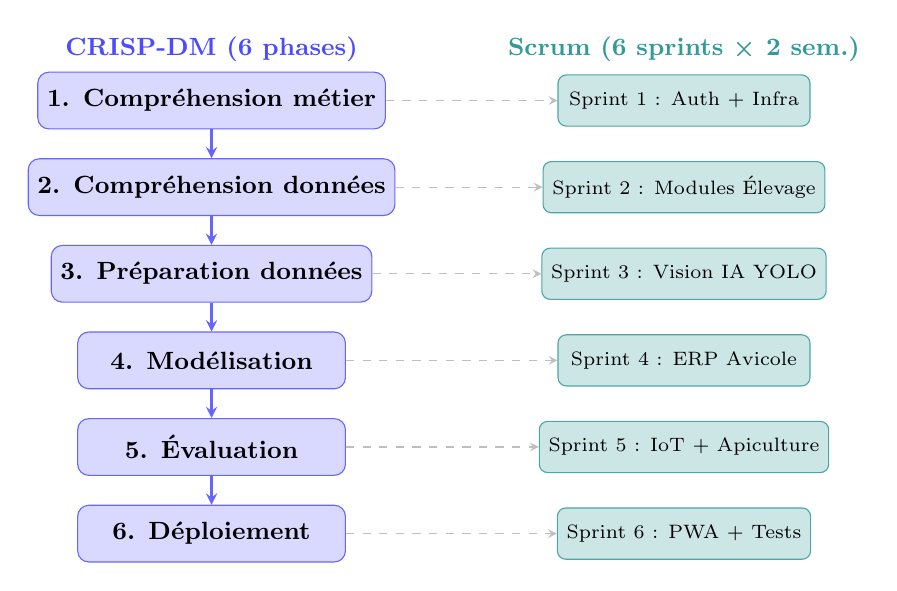
\begin{tikzpicture}[
  phase/.style={rectangle, rounded corners=4pt, minimum width=3.4cm,
                minimum height=0.72cm, text centered, font=\small\bfseries,
                draw=blue!60, fill=blue!15},
  sprint/.style={rectangle, rounded corners=3pt, minimum width=3.2cm,
                 minimum height=0.65cm, text centered, font=\scriptsize,
                 draw=teal!70, fill=teal!20},
  arr/.style={->, >=stealth, thick, blue!60},
  link/.style={->, >=stealth, gray!50, dashed},
]
\node[phase] (c1) at (0,0)    {1. Compréhension métier};
\node[phase] (c2) at (0,-1.1) {2. Compréhension données};
\node[phase] (c3) at (0,-2.2) {3. Préparation données};
\node[phase] (c4) at (0,-3.3) {4. Modélisation};
\node[phase] (c5) at (0,-4.4) {5. Évaluation};
\node[phase] (c6) at (0,-5.5) {6. Déploiement};

\draw[arr] (c1)--(c2); \draw[arr] (c2)--(c3);
\draw[arr] (c3)--(c4); \draw[arr] (c4)--(c5); \draw[arr] (c5)--(c6);

\node[sprint] (s1) at (6,0)    {Sprint 1 : Auth + Infra};
\node[sprint] (s2) at (6,-1.1) {Sprint 2 : Modules Élevage};
\node[sprint] (s3) at (6,-2.2) {Sprint 3 : Vision IA YOLO};
\node[sprint] (s4) at (6,-3.3) {Sprint 4 : ERP Avicole};
\node[sprint] (s5) at (6,-4.4) {Sprint 5 : IoT + Apiculture};
\node[sprint] (s6) at (6,-5.5) {Sprint 6 : PWA + Tests};

\draw[link] (c1.east)--(s1.west); \draw[link] (c2.east)--(s2.west);
\draw[link] (c3.east)--(s3.west); \draw[link] (c4.east)--(s4.west);
\draw[link] (c5.east)--(s5.west); \draw[link] (c6.east)--(s6.west);

\node[font=\small\bfseries, blue!70]  at (0, 0.65)  {CRISP-DM (6 phases)};
\node[font=\small\bfseries, teal!80]  at (6, 0.65)  {Scrum (6 sprints × 2 sem.)};
\end{tikzpicture}
\caption{Alignement des 6 phases CRISP-DM avec les 6 sprints Scrum du projet Smart Farm AI v3.0}
\label{fig:crisp_scrum}
\end{figure}

\subsection{Scrum adapté}

\begin{table}[H]
\centering
\caption{Product Backlog Smart Farm AI (user stories prioritaires)}
\label{tab:product_backlog}
\begin{tabularx}{\linewidth}{clXcc}
\toprule
\textbf{ID} & \textbf{Acteur} & \textbf{User Story} & \textbf{Prio} & \textbf{SP} \\
\midrule
US-01 & Éleveur  & Visualiser le dashboard ferme avec alertes temps réel & Must & 8 \\
US-02 & Éleveur  & Analyser une image d'animal avec l'IA YOLO + conseil Darija & Must & 13 \\
US-03 & Éleveur  & Gérer les lots avicoles (FCR, mortalité, ponte, vente) & Must & 13 \\
US-04 & Éleveur  & Surveiller les ruches via télémétrie IoT & Must & 8 \\
US-05 & Worker   & Consulter les tâches assignées depuis l'app mobile offline & Must & 5 \\
US-06 & Worker   & S'authentifier par OTP WhatsApp sans mot de passe & Must & 5 \\
US-07 & Éleveur  & Localiser vétérinaires et marchés sur la carte GIS & Should & 5 \\
US-08 & Éleveur  & Recevoir des alertes d'urgence sur WhatsApp & Should & 8 \\
US-09 & Éleveur  & Exporter rapports en PDF (production, finances) & Could & 3 \\
US-10 & Éleveur  & Consulter prévisions météo intégrées dans le dashboard & Could & 3 \\
\midrule
\multicolumn{4}{r}{\textbf{Total Story Points}} & \textbf{71} \\
\bottomrule
\end{tabularx}
\end{table}

\begin{table}[H]
\centering
\caption{Planification des sprints Smart Farm AI}
\label{tab:sprints}
\begin{tabularx}{\linewidth}{clXc}
\toprule
\textbf{Sprint} & \textbf{Période} & \textbf{Objectif principal} & \textbf{SP} \\
\midrule
S1 & Sem. 1--2  & Infrastructure : FastAPI, BDD PostgreSQL, Auth JWT/OTP & 13 \\
S2 & Sem. 3--4  & Gestion fermes, animaux, travailleurs ; RBAC & 13 \\
S3 & Sem. 5--6  & Module YOLO + Agent Darija RAG/LLM & 13 \\
S4 & Sem. 7--8  & ERP avicole + modèles ML (FCR, mortalité, ponte) & 13 \\
S5 & Sem. 9--10 & IoT ESP32, MQTT, WebSocket temps réel ; module apiculture & 13 \\
S6 & Sem. 11--12& PWA Worker, GIS, tests, déploiement Docker+Caddy & 6 \\
\midrule
\multicolumn{3}{r}{\textbf{Total}} & \textbf{71} \\
\bottomrule
\end{tabularx}
\end{table}

\subsection{Planification — Diagramme de Gantt}

\begin{figure}[H]
\centering
\begin{ganttchart}[
  x unit=0.78cm,
  y unit chart=0.65cm,
  vgrid,
  hgrid,
  title label font=\small\bfseries,
  bar label font=\small,
  group label font=\small\bfseries,
  milestone label font=\small\itshape,
  bar/.style={fill=blue!45, rounded corners=2pt},
  bar height=0.55,
  group/.style={fill=green!35, draw=green!70},
  milestone/.style={fill=red!65, rounded corners=2pt},
  title/.style={fill=blue!15, draw=none}
]{1}{12}
  \gantttitle{Smart Farm AI — Planification 12 semaines}{12} \\
  \gantttitle{S1}{1}\gantttitle{S2}{1}\gantttitle{S3}{1}\gantttitle{S4}{1}%
  \gantttitle{S5}{1}\gantttitle{S6}{1}\gantttitle{S7}{1}\gantttitle{S8}{1}%
  \gantttitle{S9}{1}\gantttitle{S10}{1}\gantttitle{S11}{1}\gantttitle{S12}{1} \\

  \ganttgroup{Phase 1 — Analyse \& Conception}{1}{3} \\
  \ganttbar{Étude de l'existant}{1}{1} \\
  \ganttbar{Analyse des besoins}{2}{2} \\
  \ganttbar{Architecture système}{3}{3} \\

  \ganttgroup{Phase 2 — Développement}{4}{10} \\
  \ganttbar{Sprint~1 : Auth + Infra}{4}{4} \\
  \ganttbar{Sprint~2 : Fermes + Animaux}{5}{5} \\
  \ganttbar{Sprint~3 : YOLO + RAG}{6}{7} \\
  \ganttbar{Sprint~4 : ERP Avicole}{8}{8} \\
  \ganttbar{Sprint~5 : IoT + Apiculture}{9}{9} \\
  \ganttbar{Sprint~6 : PWA + Tests}{10}{10} \\

  \ganttgroup{Phase 3 — Validation terrain}{11}{12} \\
  \ganttbar{Tests 7 fermes pilotes}{11}{11} \\
  \ganttbar{Analyse résultats + Rapport}{12}{12} \\

  \ganttmilestone{Rendu mémoire}{12}
\end{ganttchart}
\caption{Diagramme de Gantt du projet Smart Farm AI v3.0 (12 semaines)}
\label{fig:gantt}
\end{figure}

\subsection{Organigramme de l'entreprise d'accueil}

\begin{figure}[H]
\centering
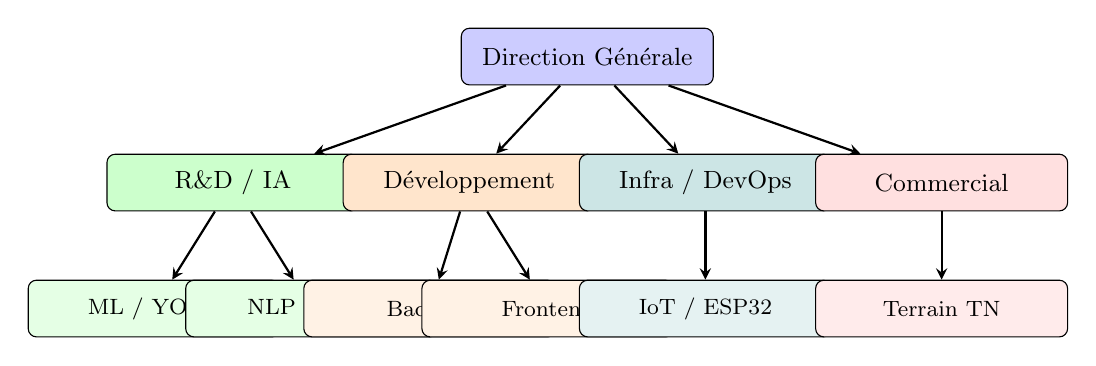
\begin{tikzpicture}[
  box/.style={draw, rounded corners=3pt, fill=#1, minimum width=3.2cm,
              minimum height=0.72cm, text centered, font=\small},
  line/.style={->, >=stealth, thick}
]
\node[box=blue!20]  (dg)  at (0,0)      {Direction Générale};
\node[box=green!20] (rd)  at (-4.5,-1.6){R\&D / IA};
\node[box=orange!20](dev) at (-1.5,-1.6){Développement};
\node[box=teal!20]  (ops) at (1.5,-1.6) {Infra / DevOps};
\node[box=red!12]   (com) at (4.5,-1.6) {Commercial};
\node[box=green!10] (ml)  at (-5.5,-3.2){\footnotesize ML / YOLO};
\node[box=green!10] (nlp) at (-3.5,-3.2){\footnotesize NLP / RAG};
\node[box=orange!10](be)  at (-2.0,-3.2){\footnotesize Backend};
\node[box=orange!10](fe)  at (-0.5,-3.2){\footnotesize Frontend};
\node[box=teal!10]  (iot) at (1.5,-3.2) {\footnotesize IoT / ESP32};
\node[box=red!8]    (sal) at (4.5,-3.2) {\footnotesize Terrain TN};
\draw[line](dg)--(rd); \draw[line](dg)--(dev);
\draw[line](dg)--(ops); \draw[line](dg)--(com);
\draw[line](rd)--(ml);  \draw[line](rd)--(nlp);
\draw[line](dev)--(be); \draw[line](dev)--(fe);
\draw[line](ops)--(iot); \draw[line](com)--(sal);
\end{tikzpicture}
\caption{Organigramme d'Intech Solutions (entreprise d'accueil)}
\label{fig:organigramme}
\end{figure}

% ── 1.4 Choix technologiques ────────────────────────────────
\section{Justification des choix technologiques}

\begin{table}[H]
\centering
\caption{Justification des choix technologiques clés}
\label{tab:choix_tech}
\begin{tabularx}{\linewidth}{lllX}
\toprule
\textbf{Domaine} & \textbf{Choix} & \textbf{Alternative} & \textbf{Justification} \\
\midrule
Backend API  & FastAPI  & Django REST & Performances async, validation Pydantic, OpenAPI auto \\
ORM          & SQLAlchemy 2.0 & Tortoise ORM & Maturité, flexibilité, support PostgreSQL+GeoAlchemy2 \\
Vision       & YOLOv8  & Detectron2  & Inférence temps réel ($<200$\,ms), pipeline Ultralytics \\
LLM local    & Ollama/Labess-7B & OpenAI API & Souveraineté, fonctionnement hors ligne, coût nul \\
LLM cloud    & Groq/Llama-3.3-70B & GPT-4 & Fallback rapide, API gratuite, multilingual \\
RAG          & ChromaDB & Pinecone    & Open-source, embarquable, compatibilité sentence-transformers \\
Frontend     & React 18 + Vite & Next.js & SPA légère, Zustand, compatibilité PWA Dexie offline \\
BDD primaire & PostgreSQL 16 & MySQL & PostGIS, transactions ACID, JSON natif \\
Protocole IoT& MQTT (Mosquitto) & HTTP poll & Légèreté, QoS niveaux, adapté aux ESP32 \\
MLOps        & MLflow  & W\&B        & Open-source, Docker-friendly, intégration DVC \\
HTTPS Proxy  & Caddy   & Nginx       & HTTPS automatique Let's Encrypt, conf minimale \\
\bottomrule
\end{tabularx}
\end{table}

\section*{Conclusion}
\addcontentsline{toc}{section}{Conclusion}
Ce chapitre a posé les fondements conceptuels et méthodologiques du projet
Smart Farm AI. L'analyse de l'existant démontre l'originalité de la plateforme
face aux solutions commerciales internationales. La méthodologie hybride
CRISP-DM/Scrum garantit à la fois la rigueur scientifique de la composante
ML et l'agilité nécessaire au développement logiciel en milieu startup.

% ============================================================
%  CHAPITRE 2 : ANALYSE DES BESOINS ET ARCHITECTURE
% ============================================================
